\section{Dictionary Learning}
\label{sec:DictionaryLearning}

Until now, we haven't given any discussion about the overcomplete dictionary $D$ that exactly leads to the sparse representations of signals.
From the definition of sparse representation, it is obvious that the choice of the dictionary will directly affect the signal processing result.

In general, this dictionary can either be chosen as a prespecified set of functions(e.g., wavelet dictionary) or designed by adapting its content to fit a given set of signal examples(e.g., \cite{aharon2006svd}).
From the performance of existing dictionary learning based works, the learned dictionaries used to outperform predefined dictionaries,
so there have been many techniques aiming to get a expressive dictionary with less computational cost.
This techniques can be directly used to deal with some geometric problem, such as compression of point cloud\cite{digne2014self}.

In this section, we also regard sparse matrix decomposition as dictionary learning.
As the name implies, sparse matrix decomposition attempts to decompose a dense matrix into the multiplication of a simple matrix(e.g., transformation matrix\cite{le2012smooth}) and the correspondent coefficient matrix which is as sparse as possible.
Generally, this decomposition is achieved with some iterative algorithm just like the dictionary learning algorithm,
so we also call the resulted simple matrix dictionary though it may not be overcomplete.

The following works show the success of dictionary learning based method in different applications.

\subsection{Linear blend skinning}
\label{subsec:LBS}

Skinning mesh animations has been an active area.
Among many proposed techniques, Linear~Blend~Skinning(LBS) is widely known to be the most popular skinning computational model due to its efficiency, simplicity, and effectiveness.
In the LBS model, skin deformation is driven by a set of bones.
Every vertex is associated with the bones via a bone-vertex weight map which quantifies the influence of each bone to the vertices.
The skin is deformed by transforming each vertex through a weighted combination of bone transformations from the rest pose.

Assume
$w_{ij}$ is the influence of $j$-th bone to the $i$-th vertex,
$p_{i}$ is the position of the $i$-th vertex at the rest pose,
$|B|$ is the number of bones, and
$R{_{j}^{t}}$ and $T{_{j}^{t}}$ are the rotation matrix and translation vector of the $j$-th bone at the $t$-th configuration, respectively,
then the deformed $i$-th vertex, $v{_{j}^{t}}$, can be computed as follows:

\small{
\begin{equation}
 \label{eq:LBS}
 v{_{j}^{t}}=\sum_{j=1}^{|B|}w_{ij}(R{_{j}^{t}}p_{i}+T{_{j}^{t}})
\end{equation}
}

By posing sparseness constraint on the weight map, the number of non-zero bone weights per vertex can be limited.
And the orthogonal constraint on $R{_{j}^{t}}$ avoids any shearing or scaling effect on the bone transformations,
thus put the transformation into rigid group.
Then the bone transformation with orthogonal rotation matrix is also called the "rigid bone".

%But the LBS model has certain limitations such as collapsing elbow and candy-wrapper effects and failure of secondary deformation.

\paragraph{(1)}
\cite{le2012smooth} introduces Smooth Skinning Decomposition with Rigid Bones(SSDR), an automated algorithm to extract the linear blending skinning, i.e., it aims to solve the inverse problem of the LBS model.

Suppose there are $|t|$ example poses of a $|V|$-vertices model, taking $\{v{_{j}^{t}}: t=1..|t|,i=1..|V|\}$ shown in () as input, SSDR decomposes them to bone transformations($R{_{j}^{t}}$, $T{_{j}^{t}}$) and the bone-vertex weight map

\small{
\begin{equation}
 \label{eq:SSDR}
 \begin{split}
 & \min_{w,R,T}E=\min_{w,R,T}\sum_{t=1}^{|t|}\sum_{i=1}^{|V|}\|v{_{j}^{t}}-\sum_{j=1}^{|B|}w_{ij}(R{_{j}^{t}}p_{i}+T{_{j}^{t}})\|^2 \\
 & s.t.~w_{ij}\ge0,~\forall i,j\\
 & ~~~~\sum_{j=1}^{|B|}w_{ij}=1,~\forall i\\
 & ~~~~|\{w_{ij}|w_{ij}\neq0\}|\le|K|,~\forall i \\
 & ~~~~{R{_{j}^{t}}}^{T}R{_{j}^{t}}=I,detR{_{j}^{t}}=1,~\forall t,j
 \end{split}
\end{equation}
}

With the sparseness constraint on the weight map, SSDR can be used for traditional skinning decomposition tasks such as animation compression and hardware-accelerated rendering.
(Figure) shows an approximation result of highly deformable model.
However, the sparseness constraint also poses certain limitations to skinning models,
e.g., it is difficult to handle exceptional vertices that are naturally associated with more than $|K|$ bones or control points.
And the relatively high computational cost makes it impractible to some degree.

\paragraph{(2)}
To address these limitations, \cite{le2013two} introduces an efficient two-layer compression technique which is formulated as a sparse dictionary learning problem. The left figure of (b) in figure..gives a clear explanation about the new technique.

Let $W\in\mathbb{R}^{k\times n}$ be the weight matrix of an input skinning model with $n$ vertices and $k$ bones, as illustrated as the top left.
At the first layer, a.k.a. $master~bone~blending$, they calculate and cache the transformations of $m$ virtual bones by blending the transformations of $k$ original bones(called $master~bones$).
At the second layer, a.k.a. $virtual~bone~blending$, they calculate the position of each vertex by blending the transformations of the virtual bones and applying the resultant transformation to the vertex.
By imposing a sparseness constraint on each blending layer, the optimization problem is formulated as

\small{
\begin{equation}
 \label{eq:TwoLayer}
 \begin{split}
 & \min_{D,A}\Delta_{W}^2=\min_{D,A}\frac{1}{kn}\|DA-W\|{_{F}^2} \\
 & s.t.~\textbf{card}(\alpha_{i})\leq2,\forall i\\
 & ~~~~~\textbf{card}(d_{i})\leq c,\forall i
 \end{split}
\end{equation}
}

By employing virtual bones to cache transformation blending of master bones,
this approach can significantly reduce computation of LBS with dense weights, with insignificant loss of accuracy of the original skinning model. Figure...
But it requires additional storage space for caching virtual bone transformations,
and transformation blending in this two-layer approach cannot go beyond certain intrinsic limitations of the LBS model,
among which sophisticated deformation effects such as muscle bulges or skin wrinkles cannot be captured well.



\vspace{15pt}
Actually, these two above methods are both not quite suitable for animation editing purposes
since their extracted bone transformations are not organized in any skeletal structures
based on which the mesh deformation is a widely-used method for animating articulated creatures such as humans and animals.
Setting up the skeleton-based animation(also known as rigging) generally consists of two main steps:
building a hierarchical skeleton with rigid bones connected by joints,
and skinning the 3D model to define how joint rotations and translations would propagate to the surface during animation.
A best result may be achieved by manually or semi-automatically repeating the two steps many times which make it costly and time-consuming.
Fortunately, the concept of using example poses can ease this problem\cite{schaefer2007example}.

\paragraph{(3)}
Attempting to take advantage of example poses, taking a set of example poses as input,
\cite{le2014ras} introduces a robust and accurate rigging framework producing its corresponding $Skeleton$-$based$ LBS model including skeletal structure, skinning weights, joint locations, and bone transformations corresponding to all the example poses.

After initializing bone transformations and determining the skeleton topology, they get the optimized LBS model by minimizing function

\small{
\begin{equation}
 \label{eq:SkeletonLBS}
 E=E_{D}+wE_{S}+\lambda E_{J}
\end{equation}
}
\\
subject to the same set of constraints () as in \cite{le2012smooth} including the \textit{sparseness~constraints}(no more than 4 non-zero weights per vertex) there and  the term $E_{D}$ is also similar to their work

\small{
\begin{equation}
 \label{eq:SRFE}
 E_{D}=\frac{1}{|t||V|}
 \sum_{t=1}^{|t|} \sum_{i=1}^{|V|}
 \|v{_{j}^{t}}
 -\sum_{j=1}^{|B|} w_{ij} ( R{_{j}^{t}}p_{i} + T{_{j}^{t}} )
 \|^2.
\end{equation}
}
\\
The term $E_{S}$ favors the smoothness of skinning weights and drives the removal of redundant bones and $E_{J}$ keeps any two connected transformations rotate around their common joint(refer to\cite{le2014ras} for the formulation).

The output can be directly used to set up skeleton-based animation in various 3D modeling and animation software as well as game engines. Despite the achieved accuracy and robustness, this approach has several limitations including the aforementioned low computational efficiency, example data dependency, and limited approximation power of the LBS model.


\begin{figure}[ht]
  \centering
  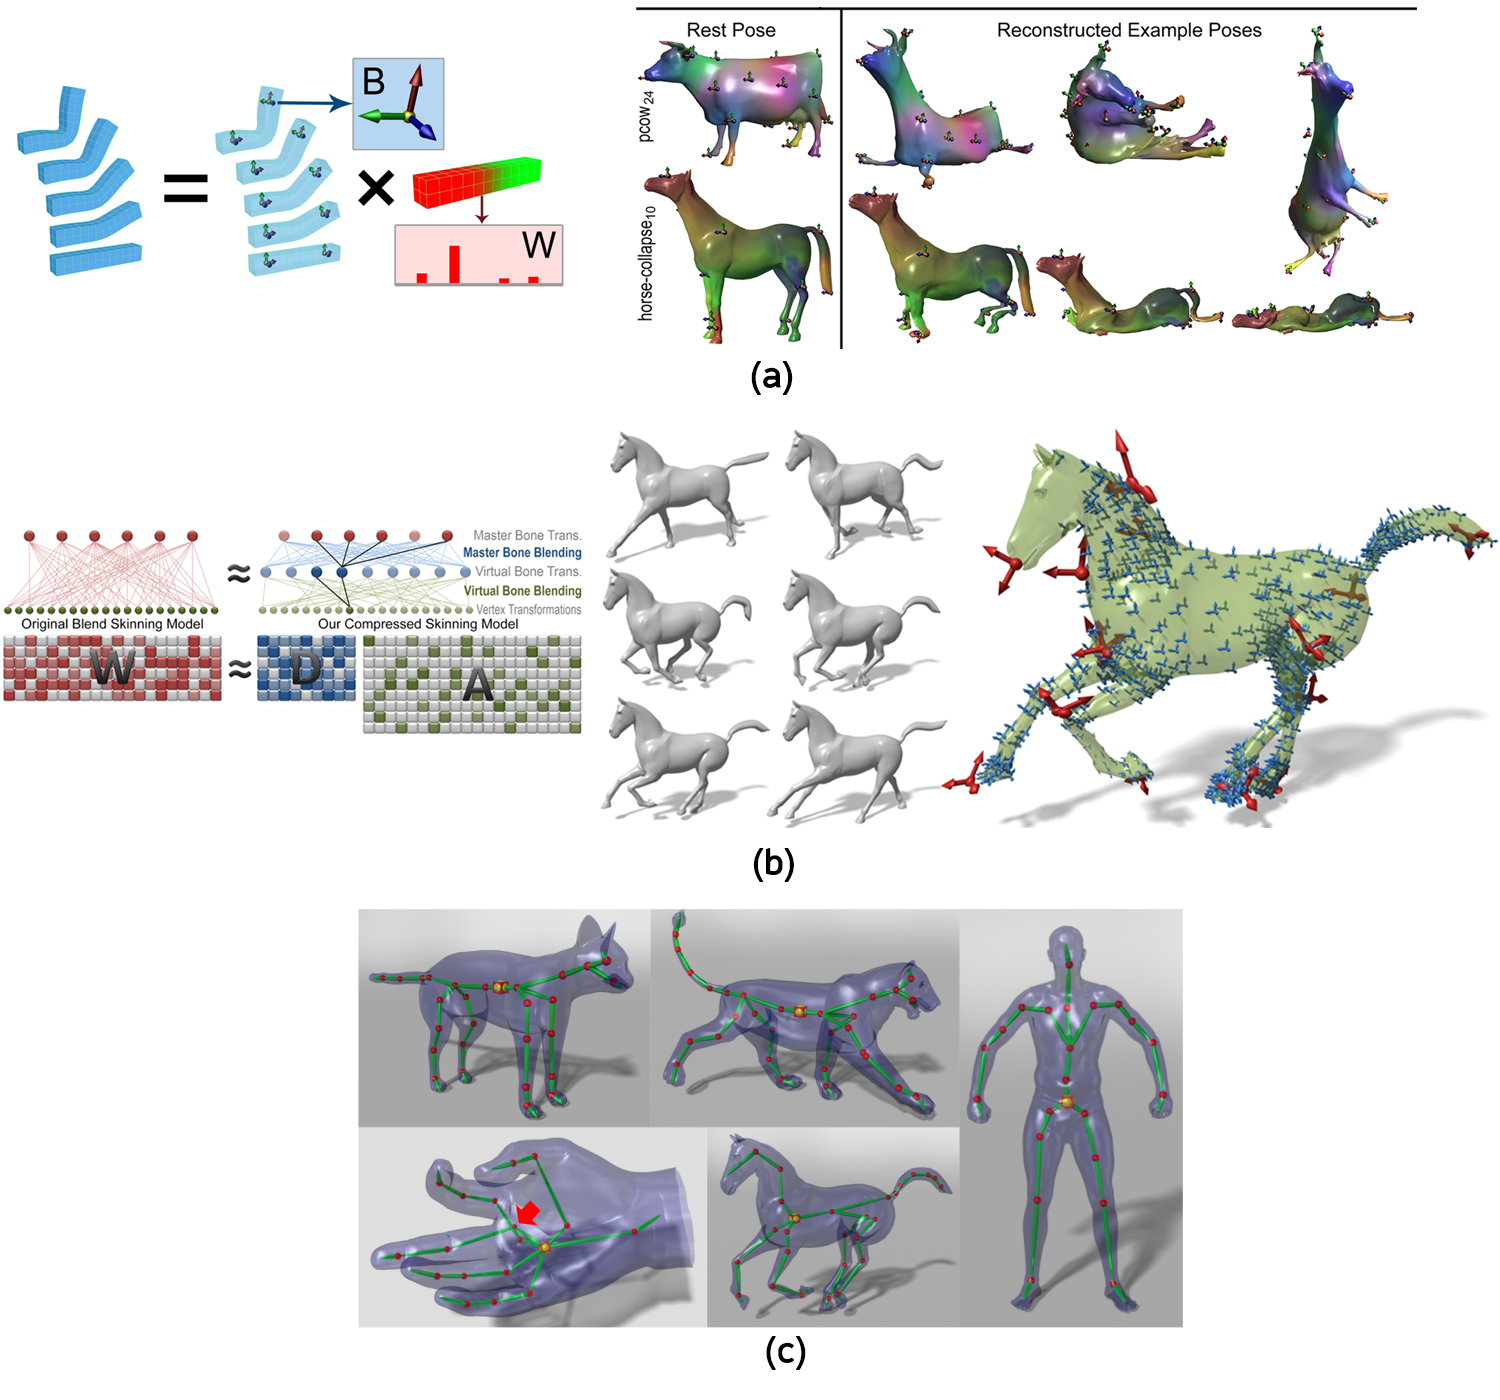
\includegraphics[width=3in]{images/skinning_decomposition}
  \caption{Dictionary learning: skinning results. (a): \cite{le2012smooth}, left: a set of example poses are decomposed into rigid bone transformation B and a sparse, convex bone-vertex weight map W. right: results of SSDR on elastic models. (b): \cite{le2013two}, left: two-layer scheme. right: an animated mesh sequence and its corresponding compressed skinning model. (c): \cite{le2014ras}, result of rigging various models such as quadrupled animals, humans, and highly deformable models.}
\end{figure}


\subsection{Deformation}
\label{subsec:deformation}


Time-varying dynamic geometry with very fine dynamic shape detail can be generated and rendered at very high visual fidelity.
When creating such content, artists usually rely on a low-dimensional control parameterization.
Despite increasing expensive power of such parameterizations and simulations, producing such realistic animations from scratch is a labor-intensive process.

As Figure.. shows, a new facial expression is generated by summing deformation components.
To decompose any mesh animations like performance faces into sparse and localized deformation modes(shown in blue),
\cite{neumann2013sparse} proposes a new efficient, easy-to-implement, and versatile data-driven approach inspired by matrix decomposition methods like sparse PCA\cite{zou2006sparse}.
Given a mesh animation with $F$ frames, each frame $f$ consists of $N$ vertices positions $\mathbf{v}{_{i}^{(f)}}$, assembling a single $'$animation matrix$'$ $X\in \mathbb{R}^{F\times 3N}$ by stacking the vertices of all frames in a row-wise fashion

\small{
\begin{equation}
 \label{eq:edgecotanoperator}
 \mathbf{X} = {\left[ \begin{array}{cccc}
 (\mathbf{v}{_1^{(1)}})^{T} & (\mathbf{v}{_2^{(1)}})^{T} & \cdots & (\mathbf{v}{_{N}^{(1)}})^{T}\\
 (\mathbf{v}{_1^{(2)}})^{T} & (\mathbf{v}{_2^{(2)}})^{T} & \cdots & (\mathbf{v}{_{N}^{(2)}})^{T}\\
 \vdots & \vdots & \ddots & \vdots\\
 (\mathbf{v}{_1^{(F)}})^{T} & (\mathbf{v}{_2^{(F)}})^{T} & \cdots & (\mathbf{v}{_{N}^{(F)}})^{T}
 \end{array}
 \right]}
\end{equation}
}

After some preprocessing for $X$, \cite{neumann2013sparse},
following the framework of \cite{zou2006sparse},
formulates the matrix factorization into $K$ deformation components $C\in \mathbb{R}_{k\times 3N}$ with weights
$W\in \mathbb{R}^{F\times K}$ as a joint regularized minimization problem

\small{
\begin{equation}
 \label{eq:sparselocal}
 \mathop{\argmin}_{W,C}\|X-W\cdot C\|{_{F}^2}+\Omega(C)~~s.t.~\mathcal{V}(W)
\end{equation}
}

Observing that each triplet in the rows of $C$ forms a three-dimensional vector $\mathbf{c}{_{k}^{(i)}}=[x,y,z]{_{k}^{(i)}}$,
every such triplet corresponds to the x, y, and z displacement of vertex i in component k.
To make the dimensions vanish simultaneously to get \textit{sparsity}, $\Omega(C)$ is formulated by acting $l_1$ norm on the lengths of the displacement vectors

\small{
\begin{equation}
 \label{eq:sparselocal}
 \Omega(C)=\sum_{k=1}^{K}\sum_{i=1}^{N}\Lambda_{ki}\|\mathbf{c}{_{k}^{(i)}}\|_2.
\end{equation}
}
\\
The spatially-varying regularization parameters $\Lambda_{ki}$ makes it possible to enforce local support for the deformation components which is and exciting innovation.

Sparse Localized Deformation components present a versatile decomposition method for space-time mesh animation data that is applicable to many settings: editing, control, scan alignment, construction of static and parametric shape models etc.
It is mentioned in this paper that several parameters in the formulation are specified by users,
but it is not clear that whether the users should have knowledge of graphics or
whether it is easy for the users to give the suitable values.

\begin{figure}[ht]
  \centering
  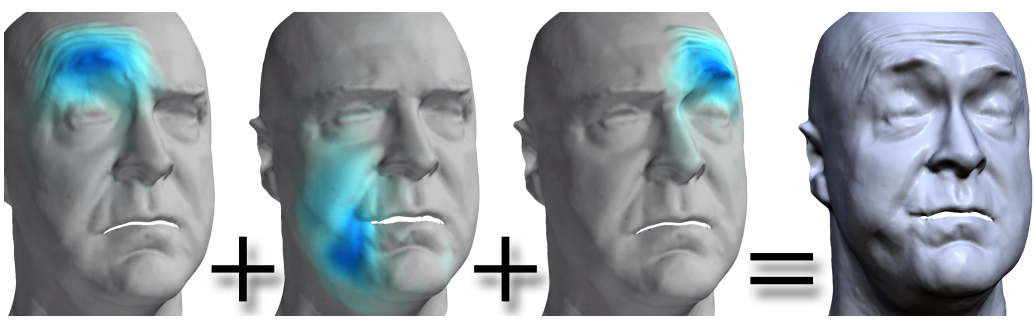
\includegraphics[width=3in]{images/localdefor_learning}
  \caption{Sparse decomposition: deformation\cite{neumann2013sparse}. A new facial expression is generated by summing deformation components, the method automatically separates spatially confined effects like separate eyebrow motions from the data.}
\end{figure}


\subsection{Reconstruction}
\label{subsec:reconstruction}

Surface reconstruction from point cloud is of great practical importance in computer graphics,
it takes as input a set of dense, unorganized points sampled from a subjacent, piecewise smooth surface and outputs a triangular mesh to approximate the surface.
Existing methods often realize reconstruction via a few phases with respective goals, e.g., as mentioned in section..., point cloud consolidation can be a preprocessing phasse to denoise, remove outlier and thus can reduce more reliable normal estimation.
However, integration of processing phases may not give an optimal solution.

To avoid the inherent limitations of multi-phase processing in the prior art, \cite{xiong2014robust} proposes a unified framework that treats geometry and connectivity construction as one joint optimization problem.

As figure..(a) shows, given a point set $\mathbb{P}=\{ \mathbf{p}_1, \mathbf{p}_2, \cdots, \mathbf{p}_n \}$(blue) sampled from a piecewise smooth surface $\textsl{S}$,
they attempt to find a triangular mesh $\textsl{M}=\{ \mathbb{V}, \mathbb{}F\}$ with
vertex set $\mathbb{V}=\{ \mathbf{v}_1, \mathbf{v}_2, \cdots, \mathbf{v}_m \}$(red) and triangle set $\mathbb{F}$ to approximate the underlying surface $\textsl{S}$ so that the approximation error is as small as possible

\small{
\begin{equation}
 \label{eq:dictreconstruction}
 \begin{split}
 & \min_{\mathbf{B},\mathbf{V}}\frac{1}{n}\sum_{i=1}^{n}\|\mathbf{p}_{i}-\mathbf{Vb}_{i}\|{_2^{q}}+E_{reg}\\
 & s.t.~\|b_{i}\|_0\le3,~\|b_{i}\|_1=1,~b_{i}\ge0,~\forall i \\
 & ~~~~~B\in \mathbb{R}^{m\times n}
 \end{split}
\end{equation}
}
\\
where $E_{reg}$ is to regularize the reconstructed mesh to produce good mesh quality,
each column of sparse coding matrix $B$ corresponds to a triangle in mesh. Finally, all the points sampled from the region approximated by a triangle can be represented as a convex combination of the same three vertices.

Figure...shows the reconstruction result, with high triangle quality, of the Merlion model with various geometric features such as sharp and semi-sharp features and different levels of surface details. Despite these high quality results, the nonconvex optimization model makes it difficult for the solver to theoretically guarantee convergence or produce a global optimal solution. And it can fail when the point cloud has large holes or is highly non-uniform due to the current sampling method.

\begin{figure}[ht]
  \centering
  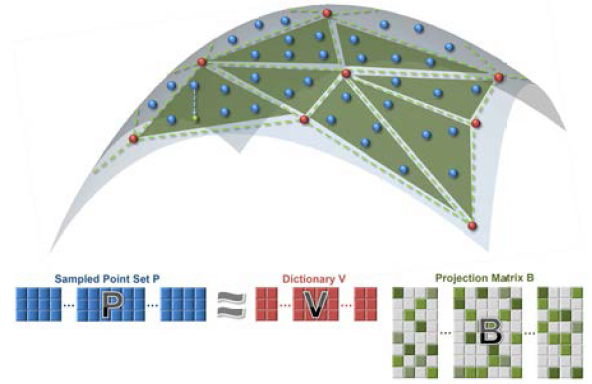
\includegraphics[width=3in]{images/reconstruction_learning}
  \caption{Dictionary learning: reconstruction\cite{}. Left: (Top)an illustration of the reconstruction problem. Given point set $\mathbb{P}$(blue) sampled from surface \textsl{S}, they approximate S with piecewise linear surface \textsl{M} with vertices $\mathbb{V}$(red) and triangles $\mathbb{F}$. (Bottom) The reconstruction problem where $P$ is the position of sample point set. $V$ is the dictionary and $B$(green) is the sparse coding matrix that encodes triangles $\mathbb{F}$. Right: reconstruction result of the Merlion model.}
\end{figure}


\subsection{Compression}
\label{subsec:compression}

\paragraph{(1)}The compression of unorganized point clouds have also attracted much attention due to the drastic improvement in scanner acquisition devices yielding point sets of tens of millions of points at high precision. But the counterpart of this development are datasets requiring ever higher storage capacity which results in the expensive cost in point cloud processing.

In \cite{digne2014self}, after selecting a subset of points(the seeds) that will serve as center points to cover the surface with local patches,
they compute patch descriptions using a new neighborhood descriptor((a) in Figure),
finally directly using the K-SVD algorithm \cite{aharon2006svd}

\small{
\begin{equation}
\label{eq:dictcompression}
\begin{split}
&\min_{D,X}  \|Y-DX\| \\
&~\mathrm{s.t.}~ \|\mathbf{x}_i\|_0 \leq s,\,\forall i
\end{split}
\end{equation}
}
\\
to exploit the self-similarity of the descriptions and build a custom dictionary $D$((b) in Figure) over which all descriptors will be decomposed sparsely with $X$.
Here $Y$ corresponds to the patch descriptions.
Briefly, selected patch descriptions deduce the dictionary.
Thus a new seed selection strategies or patch descriptors may result in higher performance,
this just tells the unrobustness of heuristic methods.
This compression is done at the resolution of the scanner enabling improved control of the point cloud resolution.
It achieves a filtering of noise whose magnitude is smaller than the scanner precision.
Figure(c) in Figure... gives one compression result.

\begin{figure}[ht]
  \centering
  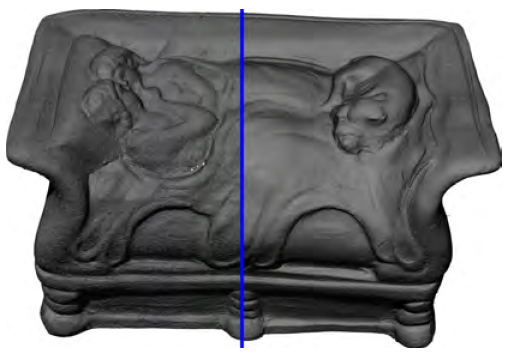
\includegraphics[width=3.0in]{images/compression_learning}
  \caption{Sparse decomposition: point cloud compression\cite{digne2014self}. (a): the local neighborhood description: a height map over a radial grid. (b): dictionary built for the Lovers(c) and the atoms are shown by order of importance(total absolute weight in the linear decompositions). (c): the Lovers(15.8 million points). By exploiting self-similarity in the model, it was compressed down to 1.15 MB. The resulting model(right) is very close to the original one(left), as the reconstruction error is less than the laser scanner precision(0.02mm) for 99.14\% of the input points.}
\end{figure}


\paragraph{(2)}
Real-time rendering of complex scenes with full global illumination is one of the main goals of computer graphics.
A popular approach is to pre-compute detailed surface light fields(SLF) describing the appearance of the objects.
However, a key problem is that an SLF data set often exhibit a very large memory footprint(often in the order of several GBs per object in the scene) and does not easily lend itself to real-time rendering.

To handle arbitrary light source configurations, general high frequency scenes and materials,
and reduce the complexity of off-line pre-computations as well as support real-time rendering,
\cite{miandji2013learning} presents a learning based algorithm for efficient compression of appearance information encoded as SLFs
which are 4D functions$f(u,v,\phi,\theta)$ represented as a \textit{hemispherical radiance distribution function}(HRDF).

After analyzing the spatial correlation in the data by clustering points with similar HRDFs,
they firstly \textit{training} a set of exemplar(basis) pairs $\{(\bar{U}_{c},\bar{V}_c)\}$ by minimizing the following energy function

\small{
\begin{equation}
 \label{eq:L1reconstruction}
 \begin{aligned}
 & E(\{\bar(U){_{a}^{c}}, \bar(V){_{a}^{c}}, \bar(S)_{ia}, M{_{ia}^{c}}\})=
   \sum_{i=1}^{} \sum_{a=1}^{}
   M{_{ia}^{c}}
   \| H{_{i}^{c}} - \bar(U){_{a}^{c}} \bar(S)_{ia} (\bar(V){_{a}^{c}})^{T}\|^2 \\
 &\mathrm{s.t.} \\
 &~~~~  (\bar(U){_{a}^{c}})^{T} \bar(U){_{a}^{c}} = (\bar(V){_{a}^{c}})^{T} \bar(V){_{a}^{c}} = I,~\forall a,\\
 &~~~~  \| \bar(S)_{ia} \|_0 \le t ~and~ \sum_{a}^{} M{_{ia}^{c}}=1,~\forall i,
 \end{aligned}
\end{equation}
}
\\
where $\bar{S}_{ia}$ contains the coefficients of the \textit{i}th HRDF when projected onto the \textit{a}th exemplar, $M$ is a binary matrix associating each HRDF to its corresponding exemplar pair$(\bar{U}{_{a}^{c}},\bar{V}{_{a}^{c}})$. Finally, let $(\xi_1, \xi_2)$ be an element of an HRDF matrix, the sparsity of $\bar{S}_i$ allows for a compact reconstruction formula for Clustered Exemplar Orthogonal Bases(CEOB)
\small{
\begin{equation}
 \label{eq:L1reconstruction}
 H{_{i}^{c}}(\xi_1, \xi_2) = \sum_{i=1}^{} \bar{U}{_{a}^{c}}(\bar{S}_{i}(t,1), \xi_1) \bar{S}_{i}(t,3) \bar(V){_{a}^{c}}(\bar{S}_{i}(t,1), \xi_2),
\end{equation}
}
\\
where $\bar{S}_{i}$ is a matrix of size $t\times3$: the first two columns describe the index of a non-zero element and the third stores its value.
Figure(b) shows three scenes with different materials.

\begin{figure}[ht]
  \centering
  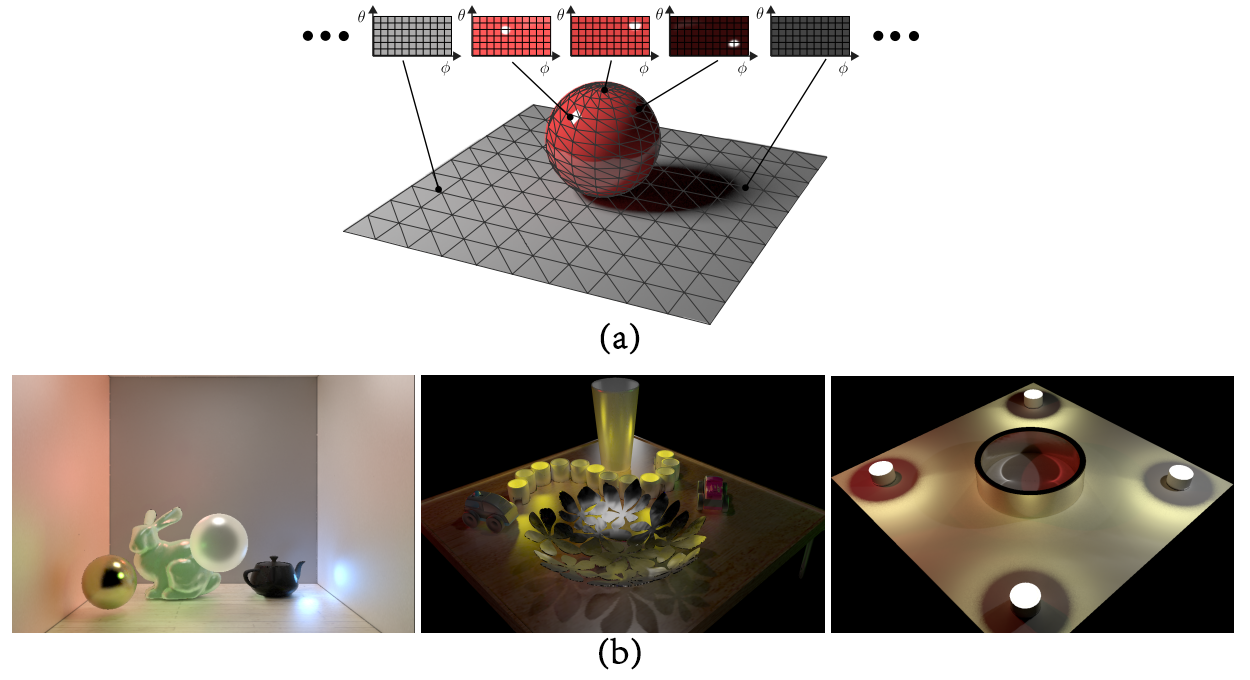
\includegraphics[width=3in]{images/rendering_learning}
  \caption{Sparse decomposition: rendering\cite{miandji2013learning}. (a): the 4D SLF function $f(u,v,\phi,\theta)$ is represented as a hemispherical radiance distribution function, HRDF. (b): rendering results using CEOB for three scenes with different materials.}
\end{figure} 